\documentclass{beamer}
\usepackage{graphicx}
\usepackage{verbatim}
\usepackage{xcolor}
\usepackage{colortbl}

\renewcommand{\figurename}{Gambar}
\renewcommand{\tablename}{Tabel}

\usetheme{metropolis}
\setbeamertemplate{navigation symbols}{}
\usepackage{listings}
\usepackage{xcolor}
\usepackage{ragged2e}

\definecolor{codegreen}{rgb}{0,0.6,0}
\definecolor{codegray}{rgb}{0.5,0.5,0.5}
\definecolor{codepurple}{rgb}{0.58,0,0.82}
\definecolor{backcolour}{rgb}{0.95,0.95,0.92}

\lstset{
    language=Java,
    backgroundcolor=\color{backcolour},   
    commentstyle=\color{codegreen},
    keywordstyle=\color{magenta},
    numberstyle=\tiny\color{codegray},
    stringstyle=\color{codepurple},
    basicstyle=\ttfamily\footnotesize,
    breakatwhitespace=false,         
    breaklines=true,                 
    captionpos=b,                    
    keepspaces=true,                 
    numbers=left,                    
    numbersep=5pt,                  
    showspaces=false,                
    showstringspaces=false,
    showtabs=false,                  
    tabsize=2,
    frame=single,
    columns=flexible
}

\addtobeamertemplate{block begin}{}{\justifying}
\addtobeamertemplate{block begin}{}{\vspace{3px}}

% Info presentasi
\title{Algoritma dan Pemrograman Komputer 1}
\subtitle{Bab 6: Struktur Kontrol 2}
\author{Aslam Pandu Tasminto -- 5002241025 \\ M. Ma'ruf Qomaruddin Kafi -- 5002241095}
\institute{Departemen Matematika \\ Fakultas Sains dan Analitika Data \\ Institut Teknologi Sepuluh Nopember}

% Logo untuk title page
\titlegraphic{%
  
\includegraphics[height=0.9cm]{../assets/logoprovikom.jpg}%
  \hspace{0.5em}%
  
\includegraphics[height=0.9cm]{../assets/logomatematika.png}%
  \hspace{0.5em}%
  
\includegraphics[height=1cm]{../assets/logoits.png}%
}

\begin{document}

% Cover
\maketitle

% Daftar Isi
\begin{frame}{Daftar Isi}
  \tableofcontents
\end{frame}

% Section 1: Pengenalan Pernyataan SWITCH
\section{Pengenalan Pernyataan SWITCH}
\begin{frame}{Pernyataan SWITCH dalam Java}
  \begin{block}{Definisi}
    Pernyataan \texttt{switch} adalah struktur kontrol percabangan yang digunakan ketika kita memiliki banyak kondisi yang identik dan ingin membandingkan suatu ekspresi dengan beberapa nilai konstan.
  \end{block}
  \begin{block}{Keunggulan SWITCH}
    \begin{itemize}
      \item Lebih rapi dan mudah dibaca dibanding multiple if-else
      \item Efisien untuk pengecekan nilai yang spesifik
      \item Mendukung berbagai tipe data: char, byte, short, int, String (JDK 7+)
    \end{itemize}
  \end{block}
\end{frame}

\begin{frame}[fragile]{Kapan Menggunakan SWITCH?}
  \begin{figure}[h]
    \centering
    \includegraphics[width=0.7\textwidth]{Struktur Kontrol 2/switch-vs-if-else.png}
    \caption{Perbandingan penggunaan SWITCH vs IF-ELSE untuk multiple conditions}
    \label{fig:switch-vs-if}
  \end{figure}
  \textbf{Sumber: }GeeksforGeeks - Switch Statements in Java
\end{frame}

% Section 2: Sintaks Dasar SWITCH
\section{Sintaks Dasar SWITCH}
\begin{frame}[fragile]{Sintaks Dasar Pernyataan SWITCH}
  \begin{block}{Struktur Dasar SWITCH}
    \begin{lstlisting}
switch (ekspresi) {
    case nilai1:
        pernyataan1;
        break;
    case nilai2:
        pernyataan2;
        break;
    case nilai3:
        pernyataan3;
        break;
    default:
        pernyataanDefault;
        break;
}
    \end{lstlisting}
  \end{block}
\end{frame}

\begin{frame}{Komponen SWITCH Statement}
  \begin{table}
    \footnotesize
    \begin{tabular}{p{0.3\textwidth}|p{0.6\textwidth}}
    \textbf{Komponen} & \textbf{Deskripsi} \\
    \hline
    \rowcolor{lightgray}
    \texttt{switch (ekspresi)} & Ekspresi yang akan dievaluasi (char, byte, short, int, String) \\
    \rowcolor{white}
    \texttt{case nilai:} & Nilai konstanta yang dibandingkan dengan ekspresi \\
    \rowcolor{lightgray}
    \texttt{pernyataan;} & Blok kode yang dieksekusi jika case match \\
    \rowcolor{white}
    \texttt{break;} & Menghentikan eksekusi dan keluar dari switch \\
    \rowcolor{lightgray}
    \texttt{default:} & Blok yang dieksekusi jika tidak ada case yang match \\
    \end{tabular}
    \caption{Komponen-komponen dalam pernyataan SWITCH}
  \end{table}
\end{frame}

\begin{frame}[fragile]{Flowchart Pernyataan SWITCH}
  \begin{figure}[h]
    \centering
    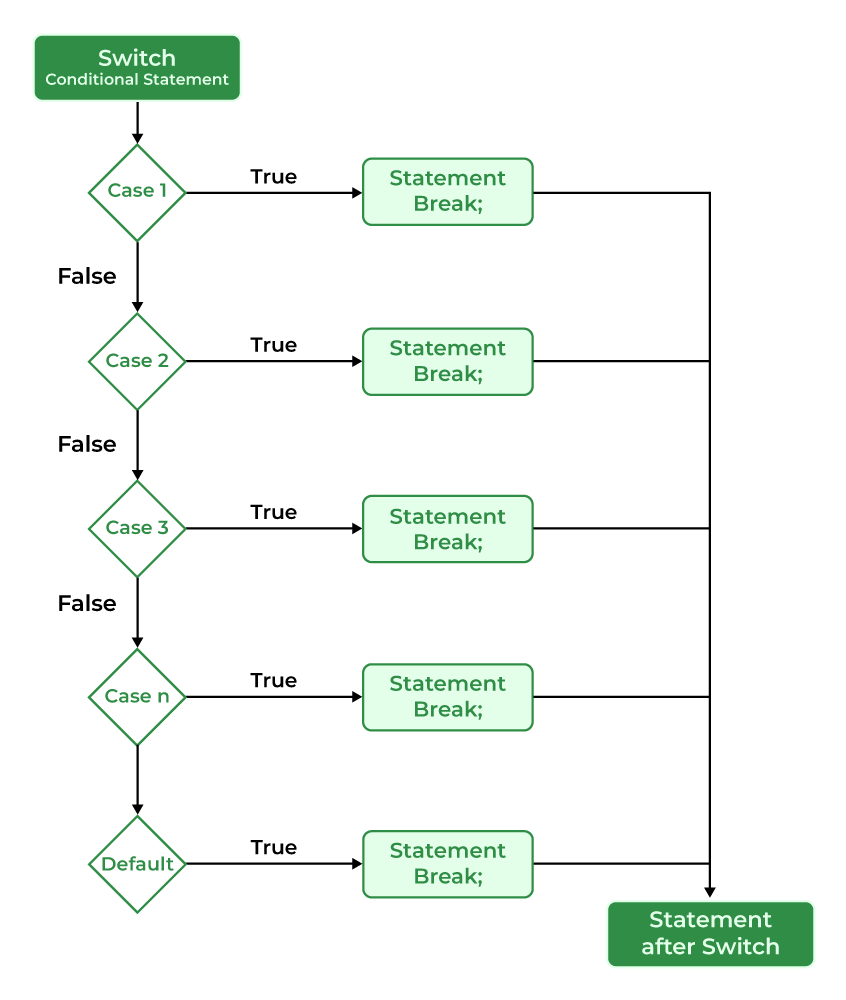
\includegraphics[width=0.65\textwidth]{Struktur Kontrol 2/switch-flowchart.png}
    \caption{Alur eksekusi pernyataan SWITCH dalam Java}
    \label{fig:switch-flowchart}
  \end{figure}
  \textbf{Sumber: }Programiz - Java switch Statement
\end{frame}

% Section 3: SWITCH dengan Tipe Data Berbeda
\section{SWITCH dengan Tipe Data Berbeda}
\begin{frame}[fragile]{SWITCH dengan Tipe Data CHAR}
  \begin{exampleblock}{Contoh Program: SWITCH dengan Char}
    \begin{lstlisting}
import java.io.IOException;

public class SwitchChar {
    public static void main(String[] args) throws IOException {
        System.out.println("Masukkan karakter nama anda");
        char inisial = (char)System.in.read();
        
        switch(inisial) {
            case 'a': 
                System.out.println("Nama anda pasti Angga");
                break;
            case 'b': 
                System.out.println("Nama anda pasti Budi");
                break;
            default: 
                System.out.println("Nama anda tidak terkenal");
                break;
        }
    }
}
    \end{lstlisting}
  \end{exampleblock}
\end{frame}

\begin{frame}{Output SWITCH dengan CHAR}
\begin{block}{Contoh Eksekusi Program}
\colorbox{gray!20}{
    \parbox{0.9\textwidth}{
        \texttt{Masukkan karakter nama anda: \textbf{a}\\
        Nama anda pasti Angga}
    }
}
\end{block}

\begin{block}{Contoh Lain}
\colorbox{gray!20}{
    \parbox{0.9\textwidth}{
        \texttt{Masukkan karakter nama anda: \textbf{c}\\
        Nama anda tidak terkenal}
    }
}
\end{block}

\begin{block}{Catatan Penting}
\begin{itemize}
\item Gunakan single quote (\texttt{' '}) untuk karakter
\item \texttt{System.in.read()} membutuhkan \texttt{throws IOException}
\item Case-sensitive: 'A' berbeda dengan 'a'
\end{itemize}
\end{block}
\end{frame}

\begin{frame}[fragile]{SWITCH dengan Tipe Data INT}
  \begin{exampleblock}{Contoh Program: Konversi Bulan}
    \begin{lstlisting}
public class SwitchInt {
    public static void main(String[] args) {
        int bulan = 8;
        String bulanString;
        
        switch (bulan) {
            case 1: bulanString = "Januari"; break;
            case 2: bulanString = "Februari"; break;
            case 3: bulanString = "Maret"; break;
            case 4: bulanString = "April"; break;
            case 5: bulanString = "Mei"; break;
            case 6: bulanString = "Juni"; break;
            case 7: bulanString = "Juli"; break;
            case 8: bulanString = "Agustus"; break;
            case 9: bulanString = "September"; break;
            case 10: bulanString = "Oktober"; break;
            case 11: bulanString = "Nopember"; break;
            case 12: bulanString = "Desember"; break;
            default: bulanString = "Bulan tidak valid"; break;
        }
        System.out.println(bulanString);
    }
}
    \end{lstlisting}
  \end{exampleblock}
\end{frame}

\begin{frame}{Output SWITCH dengan INT}
\begin{block}{Contoh Eksekusi Program}
\colorbox{gray!20}{
    \parbox{0.9\textwidth}{
        \texttt{Agustus}
    }
}
\end{block}

\begin{block}{Penjelasan}
\begin{itemize}
\item Variabel \texttt{bulan} bernilai 8
\item Program mencari case yang match dengan nilai 8
\item Ditemukan di \texttt{case 8:} dan mengeksekusi \texttt{bulanString = "Agustus"}
\item \texttt{break} menghentikan eksekusi ke case berikutnya
\end{itemize}
\end{block}
\end{frame}

\begin{frame}[fragile]{SWITCH dengan Tipe Data STRING (JDK 7+)}
  \begin{exampleblock}{Contoh Program: SWITCH dengan String}
    \begin{lstlisting}
public class SwitchString {
    public static void main(String[] args) {
        String hari = "Senin";
        String jenisHari;
        
        switch (hari.toLowerCase()) {
            case "senin": 
            case "selasa": 
            case "rabu": 
            case "kamis": 
            case "jumat": 
                jenisHari = "Hari kerja"; break;
            case "sabtu": 
            case "minggu": 
                jenisHari = "Hari libur"; break;
            default: 
                jenisHari = "Hari tidak valid"; break;
        }
        System.out.println(jenisHari);
    }
}
    \end{lstlisting}
  \end{exampleblock}
\end{frame}

% Section 4: Pentingnya BREAK Statement
\section{Pentingnya BREAK Statement}
\begin{frame}[fragile]{Konsekuensi Tanpa BREAK}
  \begin{block}{SWITCH Tanpa BREAK - Fall Through}
    \begin{lstlisting}
public class SwitchNoBreak {
    public static void main(String[] args) throws IOException {
        System.out.println("Masukkan karakter nama anda");
        char inisial = (char)System.in.read();
        
        switch(inisial) {
            case 'a': System.out.println("Nama anda pasti Angga");
            case 'b': System.out.println("Nama anda pasti Budi");
            default: System.out.println("Nama anda tidak terkenal");
        }
    }
}
    \end{lstlisting}
  \end{block}
\end{frame}

\begin{frame}{Output SWITCH Tanpa BREAK}
\begin{block}{Contoh Eksekusi Program}
\colorbox{gray!20}{
    \parbox{0.9\textwidth}{
        \texttt{Masukkan karakter nama anda: \textbf{a}\\
        Nama anda pasti Angga\\
        Nama anda pasti Budi\\
        Nama anda tidak terkenal}
    }
}
\end{block}

\begin{block}{Fenomena Fall Through}
\begin{itemize}
\item Tanpa \texttt{break}, eksekusi akan "jatuh" ke case berikutnya
\item Semua pernyataan setelah case yang match akan dieksekusi
\item Dapat dimanfaatkan untuk multiple case dengan aksi sama
\end{itemize}
\end{block}
\end{frame}

\begin{frame}[fragile]{Visualisasi Fall Through Behavior}
  \begin{figure}[h]
    \centering
    \includegraphics[width=0.8\textwidth]{Struktur Kontrol 2/switch-fall-through.png}
    \caption{Ilustrasi fall through behavior dalam SWITCH statement}
    \label{fig:switch-fall-through}
  \end{figure}
  \textbf{Sumber: }Baeldung - Java Switch Statement
\end{frame}

% Section 5: Multiple Case
\section{Multiple Case Statements}
\begin{frame}[fragile]{Multiple Case untuk Aksi yang Sama}
  \begin{exampleblock}{Contoh Program: Jumlah Hari dalam Bulan}
    \begin{lstlisting}
public class SwitchMultipleCase {
    public static void main(String[] args) {
        int bulan = 2;
        int tahun = 2000;
        int jmlHari = 0;

        switch (bulan) {
            case 1: case 3: case 5: case 7: 
            case 8: case 10: case 12:
                jmlHari = 31;
                break;
            case 4: case 6: case 9: case 11:
                jmlHari = 30;
                break;
            case 2:
                if (((tahun % 4 == 0) && !(tahun % 100 == 0)) 
                    || (tahun % 400 == 0))
                    jmlHari = 29;
                else
                    jmlHari = 28;
                break;
            default:
                System.out.println("Bulan tidak valid.");
                break;
        }
        System.out.println("Jumlah hari = " + jmlHari);
    }
}
    \end{lstlisting}
  \end{exampleblock}
\end{frame}

\begin{frame}{Output Multiple Case}
\begin{block}{Contoh Eksekusi Program}
\colorbox{gray!20}{
    \parbox{0.9\textwidth}{
        \texttt{Jumlah hari = 29}
    }
}
\end{block}

\begin{block}{Penjelasan Logic}
\begin{itemize}
\item Bulan 2 (Februari) dengan tahun 2000 (tahun kabisat)
\item Tahun kabisat: habis dibagi 4, tapi tidak habis dibagi 100, atau habis dibagi 400
\item 2000 habis dibagi 400 → tahun kabisat → 29 hari
\end{itemize}
\end{block}
\end{frame}

% Section 6: Nested SWITCH
\section{Nested SWITCH Statements}
\begin{frame}[fragile]{Konsep Nested SWITCH}
  \begin{block}{SWITCH di dalam SWITCH}
    \begin{itemize}
      \item SWITCH statement dapat nested (bersarang)
      \item Berguna untuk menu bertingkat atau klasifikasi kompleks
      \item Perlu perhatian ekstra pada break statement
    \end{itemize}
  \end{block}

  \begin{exampleblock}{Contoh Program: Menu Bertingkat}
    \begin{lstlisting}
import java.util.Scanner;

public class NestedSwitch {
    public static void main(String[] args) {
        Scanner baca = new Scanner(System.in);
        
        System.out.println("Pilih program:");
        System.out.println("1. Konversi Bulan");
        System.out.println("2. Cek Hari dalam Bulan");
        System.out.print("Masukkan pilihan (1-2): ");
        
        int pilihan = baca.nextInt();
        
        switch(pilihan) {
            case 1:
                // switch untuk konversi bulan
                break;
            case 2:
                // switch untuk cek hari
                break;
            default: 
                System.out.println("Pilihan tidak valid");
                break;
        }
    }
}
    \end{lstlisting}
  \end{exampleblock}
\end{frame}

% Section 7: Best Practices
\section{Best Practices SWITCH}
\begin{frame}{Best Practices menggunakan SWITCH}
  \begin{alertblock}{Tips dan Rekomendasi}
    \begin{itemize}
      \item \textbf{Selalu gunakan break} kecuali untuk fall through yang disengaja
      \item \textbf{Gunakan default case} untuk menangani nilai tak terduga
      \item \textbf{Group case yang sama} untuk menghindari duplikasi kode
      \item \textbf{Pertimbangkan readability} - jika terlalu kompleks, gunakan if-else
      \item \textbf{Validasi input} sebelum masuk ke switch statement
    \end{itemize}
  \end{alertblock}

  \begin{block}{Kapan Memilih SWITCH vs IF-ELSE?}
    \begin{itemize}
      \item \textbf{SWITCH}: Untuk equality check dengan nilai konstan yang terbatas
      \item \textbf{IF-ELSE}: Untuk range check, kondisi kompleks, atau banyak kondisi
    \end{itemize}
  \end{block}
\end{frame}

\begin{frame}{Perbandingan SWITCH vs IF-ELSE IF}
  \begin{table}
    \footnotesize
    \begin{tabular}{p{0.45\textwidth}|p{0.45\textwidth}}
    \textbf{SWITCH Statement} & \textbf{IF-ELSE IF Statement} \\
    \hline
    \rowcolor{lightgray}
    Equality check dengan konstanta & Range check dan kondisi kompleks \\
    \rowcolor{white}
    Lebih rapi untuk banyak kondisi & Lebih fleksibel untuk logika kompleks \\
    \rowcolor{lightgray}
    Potensi lebih efisien & Mudah untuk menambahkan kondisi baru \\
    \rowcolor{white}
    Harus break secara eksplisit & Tidak perlu break statement \\
    \rowcolor{lightgray}
    Terbatas pada tipe data tertentu & Mendukung semua tipe data boolean \\
    \end{tabular}
    \caption{Perbandingan SWITCH vs IF-ELSE IF}
  \end{table}
\end{frame}

% Section 8: Latihan
\section{Latihan}
\begin{frame}{Latihan 1: Kalkulator dengan Validasi}
  \begin{block}{Soal 1: Kalkulator Cerdas}
    Buat program kalkulator menggunakan SWITCH yang:
    \begin{itemize}
      \item Meminta input 2 bilangan
      \item Meminta operator (+, -, *, /, \%)
      \item Menggunakan SWITCH untuk memilih operasi
      \item \textbf{Fitur validasi}:
        \begin{itemize}
          \item Untuk operator '/', cek pembagi tidak boleh 0
          \item Untuk operator '\%,' cek pembagi tidak boleh 0  
          \item Tampilkan pesan error untuk operator tidak valid
        \end{itemize}
      \item Tampilkan hasil operasi dengan format: 
        \texttt{10 + 5 = 15}
    \end{itemize}
  \end{block}
\end{frame}

\begin{frame}{Latihan 2: Sistem Klasifikasi Nilai}
  \begin{block}{Soal 2: Konversi dan Klasifikasi Nilai}
    Buat program yang mengkombinasikan IF dan SWITCH untuk:
    \begin{itemize}
      \item \textbf{Input}: nilai angka (0-100)
      \item \textbf{Step 1}: Konversi ke nilai huruf menggunakan IF-ELSE IF:
        \begin{itemize}
          \item A: 86-100, AB: 76-85, B: 66-75, BC: 61-65, C: 56-60, D: 41-55, E: 0-40
        \end{itemize}
      \item \textbf{Step 2}: Konversi ke predikat menggunakan SWITCH:
        \begin{itemize}
          \item A = Luar Biasa, B/AB = Baik, BC/C = Cukup, D/E = Perlu Improvement
        \end{itemize}
      \item \textbf{Output}: 
        \texttt{Nilai 85 → AB → Baik}
    \end{itemize}
  \end{block}
\end{frame}

\begin{frame}{Latihan 3: Sistem Menu Geometri Bertingkat}
  \begin{block}{Soal 3: Kalkulator Geometri 2 Level}
    Buat program dengan \textbf{nested SWITCH} untuk menghitung bangun ruang:
    \begin{itemize}
      \item \textbf{Menu Level 1}: Pilih bangun ruang
        \begin{itemize}
          \item 1: Lingkaran, 2: Tabung, 3: Kerucut, 4: Bola
        \end{itemize}
      \item \textbf{Menu Level 2}: Pilih perhitungan
        \begin{itemize}
          \item Lingkaran: 1-Luas, 2-Keliling
          \item Tabung: 1-Volume, 2-Luas Permukaan
          \item Kerucut: 1-Volume, 2-Luas Permukaan  
          \item Bola: 1-Volume, 2-Luas Permukaan
        \end{itemize}
      \item \textbf{Fitur}: 
        \begin{itemize}
          \item Validasi input menu
          \item Gunakan \texttt{Math.PI} untuk nilai π
          \item Tampilkan rumus yang digunakan
        \end{itemize}
    \end{itemize}
  \end{block}
\end{frame}

% Section 9: Kesimpulan
\section{Kesimpulan}
\begin{frame}{Kesimpulan}
  \begin{alertblock}{Inti Bab 6: Struktur Kontrol 2 - SWITCH}
    \begin{itemize}
      \item \textbf{SWITCH} alternatif yang elegan untuk multiple if-else
      \item Mendukung berbagai tipe data: \texttt{char, byte, short, int, String}
      \item \textbf{BREAK} statement penting untuk mencegah fall through
      \item \textbf{DEFAULT} case menangani nilai tak terduga
      \item \textbf{Multiple case} untuk grouping aksi yang sama
      \item \textbf{Nested switch} untuk menu bertingkat yang kompleks
    \end{itemize}
  \end{alertblock}
\end{frame}

% Section 10: Referensi
\section{Referensi}
\begin{frame}{Referensi}
  \begin{block}{Referensi:}
    \begin{itemize}
      \item \textbf{Modul Praktikum Algoritma dan Pemrograman - Modul 6}\\
            Departemen Matematika FSAD ITS
      \item \textbf{Oracle Java Tutorials - The switch Statement}\\
            \url{https://docs.oracle.com/javase/tutorial/java/nutsandbolts/switch.html}
      \item \textbf{GeeksforGeeks - Switch Statements in Java}\\
            \url{https://www.geeksforgeeks.org/switch-statement-in-java/}
    \end{itemize}
  \end{block}
\end{frame}

\begin{frame}{Referensi}
  \begin{block}{Referensi:}
    \begin{itemize}
      \item \textbf{Programiz - Java switch Statement}\\
            \url{https://www.programiz.com/java-programming/switch-statement}
      \item \textbf{Baeldung - Java Switch Statement}\\
            \url{https://www.baeldung.com/java-switch}
    \end{itemize}
  \end{block}
\end{frame}

% Penutup
\begin{frame}[standout]
  \Huge \textbf{Terima Kasih} \\[1.5em]
  \Large Pertanyaan dan Diskusi
\end{frame}

\end{document}